% OxCSProject

% Originally by Keith A. Gillow (gillow@maths.ox.ac.uk), 1997
% Modified by Sam Evans (sam@samuelevansresearch.org), 2007
% Modified by John McManigle (john@oxfordechoes.com), 2015
% Adapted by Ned Stevenson (edward.stevenson@cs.ox.ac.uk), 2024
%
% This version Copyright (c) 2024 Ned Stevenson
%
% Broad permissions are granted to use, modify, and distribute this software
% as specified in the MIT License included in this distribution's LICENSE file.



% TODO - The noIndentBlock terminates on a .cls but not on a .tex

% I've (John) tried to comment this file extensively, so read through it to see how to use the
% various options. Remember that in LaTeX, any line starting with a % is NOT executed. Several
% places below, you have a choice of which line to use out of multiple options (eg draft vs final,
% for PDF vs for binding, etc.) When you pick one, add a % to the beginning of the lines you don't
% want.

% I (Ned) found John's comments extremely helpful. You likely will too, and I've tried to similarly
% explain my additions to this template. However converting to the version you have before you was
% quite a change, so some of John's comments may not make sense to you. In that case, you're
% welcome to raise an issue on the GitHub or, better yet, come up with a better explanation and
% make a pull request to help all those that come after you, as I aim to do here.

% NS - Should you need to render for a different paper size (e.g., letter), you can change it here.
% You should also add the "final" option to render your project ready for submission.
\documentclass[a4paper, final]{oxcsproject}

% %%%% BIBLIOGRAPHY SETUP

% The science-type option: numerical in-text citation with references in order of appearance.
\usepackage[style=ieee, sorting=none, backend=biber, doi=false, isbn=false]{biblatex}
\newcommand*{\bibtitle}{References}

% This makes the bibliography left-aligned (not 'justified') and slightly smaller font.
\renewcommand*{\bibfont}{\raggedright\small}

% Change this to the name of your .bib file (usually exported from a citation manager like Zotero
% or EndNote).
\addbibresource{references.bib}


% Uncomment this if you want equation numbers per subsection (2.3.12), instead of per section
% (2.18): \numberwithin{equation}{subsection}

% %%%% TITLE PAGE INFORMATION Project title
\title{Project on a topic in Computer Science}

% The same candidate number as for your exams. You can find it in the student self service.
\candidateno{0000000}

\wordcount{0000}

% NS - What section you're submitting for. Part B for 3rd year, Part C for master's year.
\degree{Part B - MCompSci Computer Science}
% Term and year of submission
\degreedate{Trinity 2024}

% %%%% USEFUL PACKAGES These are some useful packages that are not critical to using this template,
% but some that you may find helpful to look into. Many are demonstrated in this document, but you
% should look into their other features as you go.

% % Load the glossary terms that you've defined in glossary.tex
%% Glossary stuff
\usepackage[acronym]{glossaries}

\makeglossaries

\newacronym{cs}{CS}{Computer Science}
\newacronym{ide}{IDE}{Integrated Development Environment}
\newacronym{vscode}{VS Code}{Visual Studio Code}


% NS - Allows you to use .svg vector images for your figures, as you should aim to do
\usepackage{svg}

% Useful for consistently formatting numbers with units (e.g., 512 kB, 20 ms, 330 mV, etc.)
\usepackage{siunitx}

% %%%% YOUR PACKAGES This is a good place for you to load and configure any extra packages you're
% using.

% \usepackage{myreallycoolpackage}

% %%%% YOUR OWN PERSONAL MACROS This is a good place to dump your own LaTeX macros as they come up.

% \newcommand{\mycommand}{Hello World!}

% %%%% THE ACTUAL DOCUMENT STARTS HERE
\begin{document}

% JEM: Pages are roman numbered from here, though page numbers are invisible until ToC. This is in
% keeping with most typesetting conventions.
\begin{romanpages}

	% JEM: By default, this template uses the traditional Oxford "Belt Crest". Un-comment the
	% following line to use the newer, "Blue Square" logo:
	% \renewcommand{\crest}{{
\includegraphics[width=4.2cm, height=4.2cm]{figures/newlogo.pdf}}}

	% Title page is created here

	% NS - Remember that your title page doesn't count towards your word count
	\maketitle

	% %%%% ACKNOWLEDGEMENTS -- Nothing to do here except comment out if you don't want it.

	% NS - Similarly, your acknowledgements don't count for your word count
	\begin{acknowledgements}
		You might want to thank your supervisor or anyone else who supported your project, your friends or
family who stayed up at night to keep you company, or the guy at your favourite coffee shop who
you saw more often than you saw your own feet.

I'd like to thank my supervisors for encouraging me to explore the power of \LaTeX\ and John
McManigle for providing such an effective and helpful starting point for this template.

	\end{acknowledgements}

	% %%%% ABSTRACT -- Nothing to do here except comment out if you don't want it.
	\begin{abstract}
		OxCSProject is a \LaTeX\ template intended to encourage you to become familiar with using \LaTeX,
give you a helpful starting point when it comes to structuring your project report, and ensure
that you have easy and consistent formatting for your project. OxCSProject is an adaptation of
very helpful work done by those intending to serve the same purpose as OxCSProject in different
aspects of Oxford academic life, and would not exist without them.

OxCSProject is also designed to be an introduction into the basic tools that I expect you'll find
helpful throughout the process of writing your report, as well as introduce you to other tools
that you may appreciate being aware of. Lastly, ways for the value of OxCSProject to be enhanced
are laid out, so that you can contribute any additional development for future students to enjoy.

	\end{abstract}

	% This aligns the bottom of the text of each page. It generally makes things look better.
	\flushbottom

	% NS - Prints out an easy to navigate list of the todos you've left in your document
	\listoftodos

	% This is where the whole-document ToC appears: NS - Again, your table of contents isn't
	% included in your word count
	\tableofcontents

	% %%%% LIST OF ABBREVIATIONS

	% NS - Prints out a list of the acronyms that you've defined in glossary.tex. Just comment it
	% out if you don't want to list the acronyms. You can still use the inline declarations.
	\printglossary[type=\acronymtype]

	% The Roman pages, like the Roman Empire, must come to its inevitable close.
\end{romanpages}

% %%%% SECTIONS Add or remove any sections you'd like here, by file name (excluding '.tex'):
\flushbottom

\section{Introduction}
\label{sec:introduction}

OxCSProject is a (hopefully) easy to use \LaTeX\ template that you can use to develop and format
your 3\textsuperscript{rd} or 4\textsuperscript{th} year \acrfull{cs} project at the University of
Oxford. This should allow you to avoid all of that silly formatting nonsense and stick to the
thing that you're really here for, your project.

This template comes as the full package, and even compiles to its own user manual, which can also
be found alongside the template on GitHub~\cite{stevensonNedStevensonOxCSProject2024} once you
inevitably start writing up your own work. However, that doesn't mean you shouldn't modify,
extend, and augment the class to fit your needs. That might mean a project for a degree that
\textit{isn't} \acrlong{cs}, updating it to match new formatting requirements, or using your own
set of packages and tools to fit your project.

If you do adapt this template to suit another purpose, such as a project for another Oxford
degree, I encourage you to publish and advertise it just like I do here.

\subsection{Motivation}

I wanted to make this template because navigating \LaTeX\ and trying to adapt and modify John's
template while I was conducting my project was one more thing that I needed to do. It was
certainly worth it, it's something I realised that I could do for your project too, as well as
ahead of my own Part C project. I'm hoping that making it easy to use \LaTeX\ in your project will
mean you choose to do so, making your project better than it otherwise would have been and helping
you develop yet another skill for your future endeavours.

\subsection{Structure of the Document}
The rest of this document is structured as follows:

Section~\ref{sec:installation} describes how to install this template to
OverLeaf~\cite{OverleafOnlineLaTeX}, an easy to use online \LaTeX\ editor. It also includes how to
install this template so that you can develop your project writeup offline if you prefer.

Section~\ref{sec:background} discusses the reasons for working with \LaTeX\ over methods of
developing your project writeup, such as Microsoft Word or Google Docs.

Section~\ref{sec:usage} demonstrates how to use some of the features of \LaTeX\ you may find helpful
to be familiar with while preparing your writeup.

Section~\ref{sec:other_tools} introduces some of the other tools that it's worth becoming
acquainted with to make your project as good as it can be.

Section~\ref{sec:future_work} explains how you, dear reader, can add to this template for the
benefit of anyone who might embark on a project in future.

\section{Installation}
\label{sec:installation}

For the purpose of your project, I strongly encourage you to use
OverLeaf~\cite{OverleafOnlineLaTeX} while you become familiar with this new and exciting
technology. Once you feel a desire to learn more about \LaTeX, such as in the summer after your
project of choice, it is worth considering writing something in a code editor or \acrshort{ide}
such as \acrfull{vscode}, as I am for this template.

\subsection{OverLeaf}
\label{sec:installation/OverLeaf}

OverLeaf (\url{www.overleaf.com}) is an online \LaTeX\ editor that makes it easy to get started
with using \LaTeX\, avoiding having to install a TeX distribution such as TeX
Live~\cite{TeXLiveTeX} onto your PC and letting you share your writeup with your supervisor to
make getting feedback as easy as possible.

As a disclaimer, these steps may not be perfectly accurate, since I'm writing them from memory and
they are, of course, subject to change.

\begin{enumerate}
	\item Navigate to \url{www.overleaf.com} and create an account using your Oxford login. Either
	      your college (e.g., your.name@college.ox.ac.uk) or your department (e.g.,
	      your.name@cs.ox.ac.uk) alias is fine, since you can later add the other as a secondary
	      email. By using an Oxford email, you will get free access to the premium features.
	\item In your user settings, link your OverLeaf account to a GitHub account.
	      \todo[inline]{Expand on this. I don't remember how this goes}
	\item Go to \url{github.com/Ned-Stevenson/OxCSProject} and create a fork of OxCSProject. This
	      will create a new repo that you own as a copy of OxCSProject, which you can then import
	      into OverLeaf.
	\item At the OverLeaf home page (\url{www.overleaf.com/project}), create a new project, and
	      select "Import from GitHub". From the list, select your forked repo.
\end{enumerate}

\subsection{Offline}
\label{sec:installation/offline}

To install offline, you need only clone this repository into whichever folder you'd like to work
in. I would recommend making a fork of the repo and cloning that so that you can version control
your work, protecting your efforts in the case of loss, damage, or theft of your favourite \LaTeX\
writing device. You will also need to install something to render your \LaTeX\ into a PDF, such as
TeX Live~\cite{TeXLiveTeX} and an \acrshort{ide} to work in.

\begin{enumerate}
	\item (Optionally) Go to \url{github.com/Ned-Stevenson/OxCSProject} and create a fork of
	      OxCSProject
	\item Clone this repo or your fork onto your local device:

	      \verb*|git clone https://github.com/Ned-Stevenson/OxCSProject.git|
	\item Install a tool such as TeX Live~\cite{TeXLiveTeX}, following any relevant instructions.
\end{enumerate}

I can also recommend the LaTeX Workshop \acrshort{vscode} extension~\cite{LaTeXWorkshopVisual} as
well as latexindent~\cite{hughesCmhughesLatexindentpl2024} to make it easy to both render your
code as well as keep it tidy and readable. Note that latexindent comes pre-installed with TeX
Live, and the configuration options that I used to format this project are available in the GitHub
repository.

\section{Background}
\label{sec:background}

\subsection{Benefits of using LaTeX}

\LaTeX\ brings all of the benefits of software development, particularly the ability to reuse work
(both your own and other people's) through the use of subroutines and packages. In \LaTeX, packages
are widely available for many different uses, some of which I try to demonstrate in
Section~\ref{sec:usage}. They are imported through the use of the \verb*|\usepackage| command, and
allow you to subsequently use the commands that they define. You can define your own subroutines
using the \verb*|\newcommand| command, helping you stay on top of keeping your documents concise
and fast to work on.

Another benefit that \LaTeX\ affords us is the separation of our work into multiple, more easily
navigated files. I found it helpful to separate my project to include one file per section, to
keep any one file where I was actually working and writing content to a manageable length. Of
course you don't need to copy me if you prefer to write your documents in a single monolithic
file, but at least you have the option.

\subsection{Challenges of working in conventional word processors}

One of the challenges of working in a word processor is the way that it can slow down as the size
of the document you're navigating grows. This can get quite frustrating, particularly as you try
to get the finishing touches on your formatting the night you're trying to submit your writeup.

Another challenge is working with automatically generated components of your document, such as
bibliographies, tables of contents, and glossaries. In \LaTeX, this type of thing can be neatly
tracked for you by whichever package you're using. And often formatting can be as simple as a
sequence of command arguments, rather than doing it manually after regenerating your tables.

And not least, displaying your code, something I hope you'll do a fair amount, feels far more
challenging in a word processor than in \LaTeX. Your only real option is to copy from your
\acrshort{ide} and keep formatting, which doesn't let you elegantly deal with long lines of code,
change your formatting after the fact, or keep your code in its source files and import it into
your document directly. All these things are handled much more elegantly in \LaTeX, as will be
demonstrated in Section~\ref{sec:code_listing}.

\section{Usage}
\label{sec:usage}

This section is intended to demonstrate some of the basic \LaTeX\ commands and features you may
find helpful to be familiar with. This is likely not a comprehensive list, so please do go looking
for other features and packages that you think you may find helpful. As with everything else,
Stack Overflow is the best teacher there is!

\subsection{Using Images}

Throughout your project writeup, you will need to include figures, such as
Figure~\ref{fig:stack_overflow} below. This is generally done using the \verb|\includegraphics{}|
command. However this doesn't include \verb|.svg| files, so the \verb|\includesvg{}| command from
the \verb|svg| library should be used in that case instead. Wherever possible, you should aim to
use vector graphic formats such as \verb|svg| or \verb|pdf| to ensure there's no chance of low
resolution, hard to read images in your writeup.

\begin{figure}[ht]
	\centering
	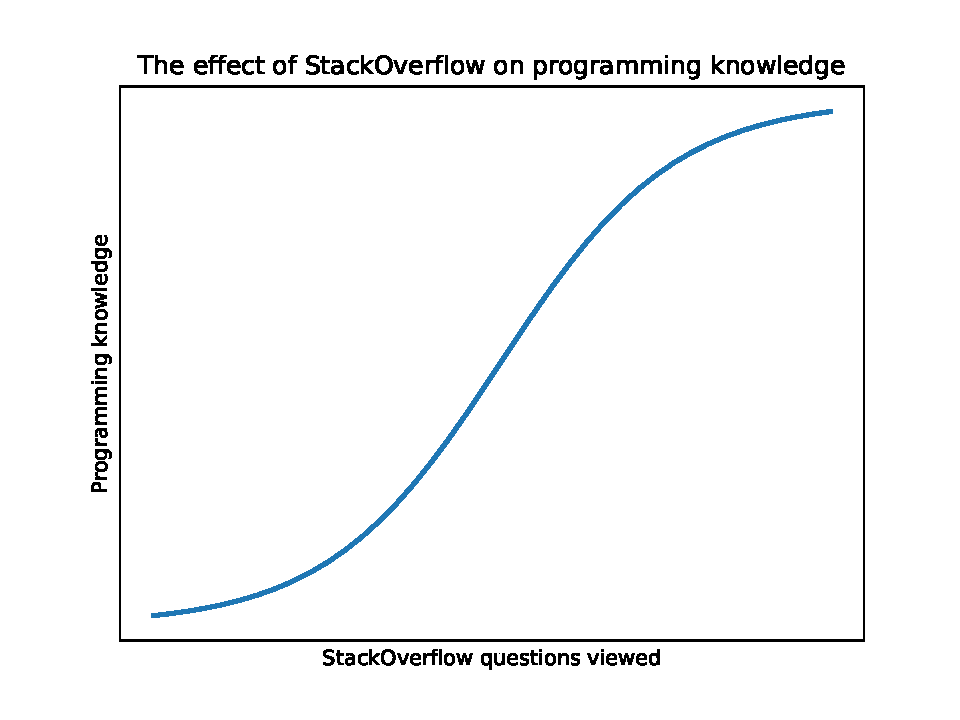
\includegraphics[width = 0.8\textwidth]{figures/stackoverflow_plot.pdf}
	\caption{A plot of \acrlong{cs} knowledge against Stack Overflow use}
	\label{fig:stack_overflow}
\end{figure}

\subsection{Using Tables}

You can see below a short list of some of the more helpful \LaTeX\ commands to know, as well as a
demonstration of how to use tables. It's okay if not all of these are helpful to you, but it may
be a good starting point for things to be aware of.

\todo[inline]{Fix latexindent on this table}
\begin{table}[ht]
	\centering
	\begin{tabular}{|p{0.15\linewidth}|p{0.70\linewidth}|}
		\hline
		\verb|\cite|  & Insert a citation using the bibliography key in your \verb|references.bib| file                              \\
		\hline
		\verb|\label| & Add a point that can be referenced elsewhere in the document, such as on a section heading, figure, or table \\
		\hline
		\verb|\ref|   & Add a reference to a label elsewhere in the document. You should precede
		this with \verb|~|, which is a whitespace that won't be split across new lines.                                              \\
		\hline
		\verb|\SI|    & Add a number formatted with SI units e.g., \verb|\SI{5}{\kilo\byte}| = \SI{5}{\kilo\byte}                    \\
		\hline
		\verb|\verb|  & An inline way to render text exactly as written in a monospace font, like the commands in this table.        \\
		\hline
	\end{tabular}
\end{table}

\subsection{Other features}

Throughout this template, I've also used a few other features that you ought to make use of, but
which weren't big enough to deserve a whole subsection. You're encouraged to go out looking for
them throughout this template to get a handle on how to use them. Some are also mentioned in the
table above with explanations of how they can be used.

\begin{itemize}
	\item Citations
	\item Acronyms
	\item References to sections and figures
	\item Lists and enumerations
\end{itemize}

\section{Other tools}
\label{sec:other_tools}

This section describes the range of tools aside from \LaTeX\ that you may want to be familiar with
while you're working on your project. This is not intended to be a comprehensive list and is only
the tools that I found useful in my project. Alternatives of course exist to everything I talk
about here, and you should investigate what works for you before simply copying my method.

\subsection{Matplotlib}

Matplotlib~\cite{MatplotlibVisualizationPython} is a Python library that provides easy to use
graph plotting functionality, along side other visualisation features that you may find helpful.
By producing your graph plots in Python, you can integrate it easily into the data processing
stage of your project, if one exists.

This lets you be very versatile with how you display your data, without needing to work within the
more constrained options of something like Microsoft Excel. I also found it more intuitive to
understand the relationships I'm trying to demonstrate when working in Python compared to a
spreadsheet.

See Figure~\ref{fig:stack_overflow} for an example of a plot made using Matplotlib, and see
appendix~\ref{sec:matplotlib_example} for source code of the plot.

\subsection{Zotero}

Zotero~\cite{ZoteroYourPersonal} is a reference manager that allows you to easily collect and keep
track of all the references that you'll need to include in your project writeup. By using the
Zotero browser extension~\cite{ZoteroConnectors} and the Better BibTeX
add-on~\cite{BetterBibTeXZotero}, you can make it easy to add to your bibliography with the
browser extension. The Better BibTeX add-on will then make sure that the citation keys that are
exported from Zotero are consistent and do not clash, making it easy to see what you're
referencing when writing your \LaTeX.

If you use this method, make sure you set the format to Better BibLaTeX when exporting to your
\verb|references.bib| file (or whatever name you end up using for your bibliography file).

\subsection{Draw.io}

Draw.io~\cite{Drawio} is a tool used to draw whatever diagrams you need to explain the core
concepts of your project. Maybe it's important to explain an inheritance diagram, relational
database, or just a simple flowchart for your code.

You can either use the online editor or download the draw.io app to use locally. You can then
export the diagrams you create to a bitmap image format, such as \verb|.png|, or to a vector
format, such as \verb|.svg|. I recommend keeping your draw.io save file in the folder with your
figures whether or not you're using an OverLeaf project.
\section{Future Work}
\label{sec:future_work}

\subsection{Things to add}

At time of writing, it doesn't feel like there are many particularly pressing missing features,
save one. I found at the end of my 3rd year project that getting a word count was much more
painful than it needed to be, since I discovered that figure captions are not included in the
built-in OverLeaf wordcount. I ended up taking the PDF produced by my \LaTeX\ and copying any text
to be included into a Word document. I then took the count that I got from that document over to
my \LaTeX\ to be re-rendered. I looked briefly for a word count library, but could find
surprisingly few packages that seemed to offer a word count, and none that I noticed were suitably
configurable to make the word count usable. If there is one you're familiar with, please read on!

For a current list of missing features and required bug fixes, please see the
\href{https://github.com/Ned-Stevenson/OxCSProject/issues}{GitHub issues page}.

\subsection{How to contribute}

If you feel that there are any features that need be added or changes to be made, please go to the
GitHub repository where you got this template and add an issue for it. And if you feel like trying
out working on open source projects, consider picking an issue and implementing it as I describe
below.

If you do want to do the work that resolving an issue would require, then make a fork of
OxCSProject in the same way as described in Section~\ref{sec:installation}. From there, you can
make whichever changes and write in whichever features you'd like. To make them available for all
to enjoy, you can then create a pull request to merge those improvements back into the template
for the next generation of Oxford Computer Scientists. This is the same process as contributing to
pretty much any open source project, and something worth trying at least once.


% % APPENDICES %% Starts lettered appendices, adds a heading in table of contents, and adds a page
% that just says "Appendices" to signal the end of your main text.
\startappendices
% Add or remove any appendices you'd like here:
\section{Code listing}
\label{sec:code_listing}

This allows us to demonstrate the code that we've written for our Project

\subsection{Demo code}

\lstinputlisting[language=Python]{text/code/myCode.py}

\subsection{Matplotlib example}
\label{sec:matplotlib_example}

\lstinputlisting[language=Python]{figures/create_plot.py}


% raggedbottom means that the bottom of the page is a bit flexible, since the line spacing inside
% the code listing is very rigid and there can be some warnings when they don't properly line up
\raggedbottom
% %%%% REFERENCES

\setlength{\baselineskip}{0pt} % JEM: Single-space References

{\renewcommand*\MakeUppercase[1]{#1}
	\printbibliography[heading=bibintoc,title={\bibtitle}]}

\end{document}
